% ============================================================
% The L2-L3 Bridge: A Bounded-Warrant Framework for Tracing
% Chip-Level Execution Conditions into AI Representations
%
% Author: Wiard Vasen
% Status: v0.1 draft, exploration
% ============================================================

\documentclass[11pt, a4paper]{article}

% --- Geometry & typography ---
\usepackage[margin=2.6cm, top=2.8cm, bottom=2.8cm]{geometry}
\usepackage[T1]{fontenc}
\usepackage[utf8]{inputenc}
\usepackage{mathpazo}
\usepackage[scaled=0.92]{helvet}
\usepackage{microtype}
\linespread{1.10}

% --- Math ---
\usepackage{amsmath, amsthm, mathtools, amssymb}
\usepackage{stmaryrd}

% --- Tables & figures ---
\usepackage{graphicx}
\usepackage{booktabs}
\usepackage{tabularx}
\usepackage{array}
\usepackage{caption}
\usepackage{tikz}
\usetikzlibrary{positioning, calc, arrows.meta}
\captionsetup{font=small, labelfont=bf, labelsep=period, justification=centering}

% --- Colors for the embedded figure ---
\definecolor{figfillL2}{HTML}{A8DDA8}
\definecolor{figfillL3}{HTML}{EBCB5A}
\definecolor{figctxBelow}{HTML}{A8C0DE}
\definecolor{figbridgered}{HTML}{B22222}
\definecolor{figbridgefill}{HTML}{F4D5D5}
\definecolor{figflowblue}{HTML}{2E5A8C}
\definecolor{figflowgreen}{HTML}{3F8B3F}
\definecolor{figflowred}{HTML}{B22222}

% --- Lists ---
\usepackage{enumitem}
\setlist{itemsep=2pt, topsep=4pt}

% --- Bibliography (natbib + bibtex) ---
\usepackage[numbers, sort&compress, square]{natbib}
\bibliographystyle{plainnat}

% --- Cross-refs ---
\usepackage{xcolor}
\definecolor{linkcol}{HTML}{1F4E79}
\definecolor{citecol}{HTML}{4A6B8A}
\usepackage[colorlinks=true, linkcolor=linkcol, urlcolor=linkcol,
            citecolor=citecol]{hyperref}

% --- Theorem environments ---
\newtheoremstyle{upldef}{6pt}{6pt}{}{}{\bfseries}{.}{0.5em}{}
\theoremstyle{upldef}
\newtheorem{definition}{Definition}
\newtheorem{postulate}{Postulate}
\newtheorem{proposition}{Proposition}
\newtheorem{remark}{Remark}

% --- Title block styling ---
\usepackage{titling}
\setlength{\droptitle}{-1.4cm}
\pretitle{\begin{center}\LARGE\bfseries}
\posttitle{\par\end{center}\vskip 0.4em}
\preauthor{\begin{center}\large}
\postauthor{\end{center}}
\predate{\begin{center}\small}
\postdate{\end{center}}

% --- Section headers: lightly stylized ---
\usepackage{titlesec}
\titleformat{\section}{\large\bfseries}{\thesection}{0.8em}{}
\titleformat{\subsection}{\normalsize\bfseries\itshape}{\thesubsection}{0.7em}{}

% --- Custom commands ---
\newcommand{\upljudge}[4]{\ensuremath{#1 \vdash #2\ @\ #3 \Leftarrow #4 : \sigma}}
\newcommand{\witness}[1]{\ensuremath{W_{\text{#1}}}}
\newcommand{\layer}[1]{\textbf{L#1}}
\newcommand{\statuslabel}[1]{\texttt{\small #1}}

% --- Title ---
\title{The L2--L3 Bridge\\[6pt]
\large\itshape A Bounded-Warrant Framework for Tracing\\
Chip-Level Execution Conditions into AI Representations}
\author{Wiard Vasen\\[2pt]\small\normalfont Independent Researcher\\\small\normalfont IJmuiden, the Netherlands}
\date{\small Draft v0.1 --- May 2026}

\begin{document}

\maketitle

% ============================================================
\begin{abstract}
\noindent
Most discussions about artificial intelligence focus either on the
semantic top of the computing stack --- prompts, outputs, alignment ---
or on the physical bottom --- timing channels, hardware faults,
side-channel leakage. The middle of the stack, where coordinated
execution turns into encoded representation, receives comparatively
little systematic attention. This paper introduces the
\emph{L2--L3 bridge} as the transition where lower-layer execution
conditions first become structurally capable of propagating into
model behaviour. We develop a \emph{bounded-warrant framework} ---
the Universal Provenance Layer (UPL) --- that adjudicates claims of
the form $\upljudge{\Gamma}{K}{B}{W}$ under stated boundary
conditions $B$ and explicit witnesses $W$. We formalise the
framework information-theoretically using conditional claim entropy
$H(K \mid W, \Gamma, B)$, the data-processing inequality, and
Fano's lower bound on adjudication error rate. We survey
chip-level calibrations --- mixed-precision arithmetic, TF32 mode,
deterministic kernels, denormal flushing, and the thermal regime
governed by Arrhenius and Johnson--Nyquist relations --- whose
configuration has been shown to influence model output. We
postulate two complementary reverse-direction modes: reverse
inference from observed AI anomalies back to candidate chip-level
causes, and \emph{toy-AI feedback}, in which a controlled small
computation produces an instrumented chip-level signature, providing
the framework's empirical entry point. The contribution is
methodological: a bounded vocabulary for talking carefully about a
zone that current AI safety and chip security literatures both
leave largely untouched.
\end{abstract}

\vspace{0.5em}
\noindent\hrulefill
\vspace{0.5em}

% ============================================================
\section{Introduction}
\label{sec:intro}

Most discussions about AI begin at the level of outputs: answers,
labels, decisions, prompts, or semantic interpretation. But AI
behaviour does not emerge directly from meaning. It emerges through
layers of execution.

At the bottom of the stack are physical execution conditions:
cache behaviour, floating-point units, DRAM, branch predictors,
memory allocation, scheduling, and timing. At the top are semantic
claims: interpretations about the world. Between those two extremes
lies a largely unexplored transition: the point where coordinated
execution becomes encoded representation. This paper focuses on
that transition. We call it the \emph{L2--L3 bridge}.

At \layer{2}, execution exists as operations, kernels, and computation
graphs. At \layer{3}, those operations crystallise into activations,
weights, attention states, and encoded vectors. The central research
question is:

\begin{quote}\itshape
Which lower-layer execution conditions, propagating through the
L2--L3 bridge, can be witnessed, mapped, checked, and ruled out
as claim-bearing for an upper-layer AI output boundary?
\end{quote}

The claim of this work is not that chip-level events directly
explain AI semantics. The claim is narrower. The L2--L3 transition
\emph{may} be the first place where lower-layer execution conditions
become structurally capable of propagating into model behaviour.
This transition therefore defines what we call the
\emph{bounded-warrant gap}: the zone between physical execution
and semantic interpretation, where claims about AI behaviour must
first become traceable, checkable, and bounded.

The contribution of this paper is methodological. We do not
present new empirical results about chip-AI propagation. We
introduce a vocabulary --- the bounded-warrant framework ---
in which such results can be stated without overclaim, and a
research question that delimits the relevant scope. The framework
is informed in spirit by Tanenbaum's MINIX discipline
\citep{tanenbaum1987}: small, clean, safe, understandable
infrastructure beneath every claim.

\paragraph{Outline.}
Section~\ref{sec:stack} characterises the AI-on-chip stack.
Section~\ref{sec:framework} introduces the bounded-warrant judgment
form. Section~\ref{sec:logictable} presents the UPL logic table
that adjudicates status assignments. Section~\ref{sec:entropy}
formalises the framework information-theoretically, including
Fano's lower bound on adjudication error.
Section~\ref{sec:bridge} concentrates on the L2--L3 bridge and
presents the main figure. Section~\ref{sec:calibrations} surveys
chip-level calibrations whose configuration is known to influence
model output, including the thermal regime.
Section~\ref{sec:reverse} states two postulates: reverse inference
from observed anomalies to chip-level candidates, and toy-AI
feedback as the framework's empirical entry point.
Section~\ref{sec:discussion} discusses open questions.

% ============================================================
\section{The Layered AI-on-Chip Stack}
\label{sec:stack}

We adopt a six-layer model of AI-on-chip execution. Each layer
corresponds to a distinct \emph{meaning-giving act} performed on
the signal as it ascends:

\begin{itemize}
\item \layer{0} \textbf{Occurrence}.\ FPU operations, cache lines,
DRAM accesses, branch predictor state. Physical execution
conditions; pre-meaning.
\item \layer{1} \textbf{Coordination}.\ Scheduling, memory
allocation, drivers, OS. The event becomes a resource-mediated
process.
\item \layer{2} \textbf{Operation}.\ Kernels, ops, computation
graphs. The coordinated process becomes a named operation.
\item \layer{3} \textbf{Representation}.\ Activations, weights,
attention, encoded state. The operation crystallises into
encoded state.
\item \layer{4} \textbf{Decision}.\ Logits, tokens, labels, output
commitment. The representation becomes a committed position.
\item \layer{5} \textbf{Interpretation}.\ Semantic claims, prompts,
tasks, world meaning. The output becomes a claim about the world.
\end{itemize}

\noindent
The meaning-making chain reads, from physical occurrence to
semantic claim:
\[
\text{Occurrence}
\;\to\;\text{Coordination}
\;\to\;\text{Operation}
\;\to\;\text{Representation}
\;\to\;\text{Decision}
\;\to\;\text{Interpretation}.
\]

The naming scheme is deliberately functional: each layer is
named for what \emph{happens} there, not for the technology used
to implement it. PyTorch, TensorFlow, and JAX all instantiate
\emph{Operation} at \layer{2}, regardless of which framework is
chosen. This decoupling matters for bounded warrants:
a witness at \layer{2} need not commit to a specific framework
to remain valid across re-implementations.

The reader should note where existing research traditions sit on
this stack. AI safety scholarship typically operates at
\layer{4}--\layer{5}: outputs, alignment, interpretation
\citep{hendrycks2021}. Chip security research typically operates
at \layer{0}--\layer{1}: timing channels, speculative execution,
microarchitectural state \citep{kocher2019, lipp2018}.
The middle of the stack --- \layer{2} and \layer{3} ---
is comparatively unaudited. This is the bounded-warrant gap.

% ============================================================
\section{The Bounded-Warrant Framework}
\label{sec:framework}

The Universal Provenance Layer (UPL) introduces a judgment form
that adjudicates claims about behaviour without asserting their
truth.

\begin{definition}[UPL judgment]\label{def:judgment}
A UPL judgment is an expression
\[
\Gamma \;\vdash\; K \;@\; B \;\Leftarrow\; W \;:\; \sigma
\]
where $\Gamma$ is a set of stated assumptions, $K$ is the claim,
$B$ is the boundary within which $K$ is asserted, $W$ is the
witness offered in support, and $\sigma \in \Sigma$ is the
status returned by adjudication.
\end{definition}

The judgment is not a proof. UPL does not validate truth; it
\emph{adjudicates admissibility}. Adjudication returns one of
nine statuses (Section~\ref{sec:logictable}). The framework
distinguishes a candidate \emph{UPLJudgment} (the input) from
the adjudicated \emph{UPLDecision} (the output).

For claims about how a lower-layer condition affects an
upper-layer output boundary, we require a structured witness
composed of six components:

\begin{definition}[Layer-effect claim]\label{def:layereffect}
A layer-effect claim is a UPL judgment
\[
\Gamma \;\vdash\; K_{\text{layer-effect}} \;@\; B
\;\Leftarrow\;
\bigl(\witness{input} \oplus \witness{exec} \oplus \witness{map}
\oplus \witness{contract} \oplus \witness{check} \oplus \witness{ruleout}\bigr)
\;:\; \sigma
\]
where the witness components are:
\begin{itemize}
\item $\witness{input}$ --- the input or workload condition under which the claim is asserted;
\item $\witness{exec}$ --- observation of the lower-layer execution condition itself;
\item $\witness{map}$ --- the mapping from execution condition to an upper-layer model variable;
\item $\witness{contract}$ --- the semantic contract that fixes what counts as the upper-layer output boundary;
\item $\witness{check}$ --- the controlled comparison demonstrating an output-boundary shift;
\item $\witness{ruleout}$ --- the evidence excluding alternative attributions of the shift.
\end{itemize}
\end{definition}

\noindent
All six components are mandatory. A layer-effect claim with
fewer than six receives status \statuslabel{incomplete}; UPL
does not award partial credit. This is the discipline that
prevents an execution trace alone --- which contains no model
information --- from being claimed as supporting a behavioural
conclusion.

\begin{remark}
Observation is not claim. Trace is not truth. No claim travels
farther than its evidence.
\end{remark}

% ============================================================
\section{The UPL Logic Table}
\label{sec:logictable}

UPL adjudicates each judgment into one of nine statuses.
Table~\ref{tab:logic} states the vocabulary, its witness condition,
and what may and may not follow.

\renewcommand{\arraystretch}{1.3}
\begin{table}[t]
\centering
\caption{UPL adjudication statuses ($\sigma \in \Sigma$).}
\label{tab:logic}
\small
\begin{tabularx}{\textwidth}{l X X}
\toprule
\textbf{Status} & \textbf{Witness condition} & \textbf{Adjudication result} \\
\midrule
\statuslabel{unsupported}      & No witness offered or no witness within $B$.                         & Claim is not admissible. \\
\statuslabel{observed}         & $\witness{exec}$ present; other components absent.                   & Descriptive claim only; no behavioural conclusion. \\
\statuslabel{witnessed}        & Witness components present and self-consistent.                      & Admissible at the witness level; no check yet. \\
\statuslabel{pending\_check}   & $\witness{check}$ specified but not yet executed.                    & Awaiting controlled comparison. \\
\statuslabel{checked}          & All six components present and check succeeded.                      & Claim admitted within $B$. \\
\statuslabel{failed}           & All six components present; check did not support $K$.              & $K$ not supported by $W$ in $B$. Not equivalent to $\neg K$. \\
\statuslabel{disputed}         & Conflicting witnesses or contested $\Gamma$.                         & Adjudication suspended pending resolution. \\
\statuslabel{incomplete}       & Required witness components missing.                                 & Cannot yet be adjudicated. \\
\statuslabel{out\_of\_boundary} & Witness lies outside $B$.                                            & Claim falls outside stated scope. \\
\bottomrule
\end{tabularx}
\end{table}

The crucial distinction is between \statuslabel{failed} and
$\neg K$. A failed check means the witness/check relation did not
support $K$ inside $B$; it does \emph{not} mean $K$ has been
disproved. Negation is itself a claim and requires its own
witness chain.

% ============================================================
\section{An Information-Theoretic Formulation}
\label{sec:entropy}

The qualitative status vocabulary of Section~\ref{sec:logictable}
admits an information-theoretic interpretation along lines familiar
from Shannon \citep{shannon1948} and the subsequent literature on
mutual information \citep{cover2006}.

\subsection{Claim entropy and witness information gain}

Let $K$ be a binary random variable whose value is the truth of
the claim under $\Gamma$ and $B$. Before any witness is offered,
the uncertainty about $K$ is the prior claim entropy
\[
H(K \mid \Gamma, B) \;=\; -\!\!\sum_{k \in \{0,1\}}
\Pr(K=k \mid \Gamma, B)\,\log_2 \Pr(K=k \mid \Gamma, B).
\]
A witness $W$ reduces this uncertainty to the conditional entropy
$H(K \mid W, \Gamma, B)$. The information gained by adjudicating
$W$ is the mutual information
\begin{equation}
I(K; W \mid \Gamma, B)
\;=\;
H(K \mid \Gamma, B) - H(K \mid W, \Gamma, B).
\label{eq:gain}
\end{equation}
We say a witness is \emph{claim-bearing} for $K$ in $B$ when
$I(K; W \mid \Gamma, B) > \tau$ for some pre-stated threshold
$\tau > 0$. The threshold is part of the boundary $B$, not a
free parameter: $B$ must specify what counts as adequate
information transfer before any check is run.

Three UPL statuses correspond naturally:
\begin{itemize}
\item \statuslabel{checked}: $I(K;W) > \tau$ and the sign of the
update supports $K$.
\item \statuslabel{failed}: $I(K;W) > \tau$ and the sign of the
update opposes $K$.
\item \statuslabel{incomplete}: $I(K;W) < \tau$.
\end{itemize}
The remaining statuses correspond to violations of well-formedness
(boundary, consistency, completeness) and are not reducible to
information-theoretic quantities alone.

\subsection{Inter-layer mutual information}

Let $X_i$ denote the random variable describing the state at layer
\layer{i}. For a propagation chain
$X_0 \to X_1 \to \cdots \to X_5$, the data-processing inequality
\citep{cover2006} gives
\begin{equation}
I(X_0; X_5)
\;\leq\;
\min_{0 \leq i < 5}\, I(X_i; X_{i+1}).
\label{eq:dpi}
\end{equation}
The bound says: the amount of \layer{0} information reaching
\layer{5} cannot exceed the narrowest channel along the path.
If any single inter-layer channel has low mutual information, no
fine-grained \layer{0} condition can survive to \layer{5}.

\subsection{The L2--L3 transition as channel}

Within this framing, the L2--L3 transition is itself a channel,
denoted $\mathcal{C}_{2\to 3}: X_2 \to X_3$, whose capacity
$C(\mathcal{C}_{2\to 3})$ bounds how much \layer{2}-level
operational detail can be encoded into \layer{3}-level
representational state.

\begin{proposition}[Bridge bottleneck]\label{prop:bottleneck}
For a propagation chain $X_0 \to \cdots \to X_4$ in which
$\mathcal{C}_{2\to 3}$ is the unique non-trivial bottleneck,
\[
I(X_0; X_4) \;\leq\; C(\mathcal{C}_{2\to 3}).
\]
\end{proposition}

\noindent
Proposition~\ref{prop:bottleneck} is a corollary of \eqref{eq:dpi}
and provides a precise sense in which the L2--L3 bridge is
informationally decisive. Where the bridge is narrow ---
e.g.\ aggressive quantisation, dimensionality collapse,
attention masking --- chip-level conditions cannot propagate
finely. Where it is wide --- e.g.\ high-precision matmul with
preserved fan-out --- they can. The framework does not assert
either condition holds in any specific deployment; it states
the structural relation.

\subsection{Lower bound on error rate from Fano's inequality}

Information-theoretic constraints also give us a lower bound on
\emph{how often} an adjudication can be in error. Fano's
inequality \citep{fano1961, cover2006} relates the conditional
entropy $H(K \mid W)$ to the probability $P_e$ of incorrect
adjudication. For a binary claim $K \in \{0, 1\}$:
\begin{equation}
H(K \mid W, \Gamma, B) \;\leq\; H_b(P_e),
\label{eq:fano}
\end{equation}
where $H_b(p) = -p\log_2 p - (1-p)\log_2(1-p)$ is the binary
entropy function. Equivalently,
\begin{equation}
P_e \;\geq\; H_b^{-1}\bigl(H(K \mid W, \Gamma, B)\bigr),
\label{eq:fano-rearranged}
\end{equation}
where $H_b^{-1}$ denotes the inverse of $H_b$ on $[0, 1/2]$.

The interpretation is operational: if the witness leaves the claim
sufficiently uncertain --- that is, if $H(K \mid W, \Gamma, B)$
is large --- then no adjudication procedure can drive $P_e$ below
the bound. Adjudicating a claim with a weak witness will be wrong
some of the time, and the lower bound on that error rate is set
by information, not by adjudicator ingenuity. This is one of the
strongest formal motivations for the bounded-warrant discipline:
constructing $W$ with high mutual information is not optional,
because $P_e$ is rate-limited by $H(K \mid W)$ regardless of how
the adjudication is implemented.

\begin{remark}
Fano's bound applies to the adjudicator viewed as a decoder of $K$
from $W$. UPL is not a decoder in the cryptographic sense, but
the structural relation holds: insufficient information cannot be
compensated for by procedure.
\end{remark}

% ============================================================
\section{The L2--L3 Bridge}
\label{sec:bridge}

Figure~\ref{fig:bridge} situates the bridge within the stack and
labels the bounded-warrant framework as a four-stage discipline.

\begin{figure}[!t]
\centering
\resizebox{0.68\textwidth}{!}{%
\begin{tikzpicture}[
  font=\sffamily,
  figlayerprimary/.style={
    rectangle, draw=black!60, thick,
    minimum width=14cm, minimum height=2.6cm,
    text width=13.4cm, align=left, inner sep=14pt, rounded corners=5pt,
  },
  figlayercontext/.style={
    rectangle, draw=black!45, thick,
    minimum width=14cm, minimum height=1.5cm,
    text width=13.4cm, align=center, inner sep=10pt, rounded corners=5pt,
  },
  figbridgebox/.style={
    rectangle, draw=figbridgered, line width=2pt, fill=figbridgefill,
    minimum width=14cm, minimum height=3cm,
    text width=13.4cm, align=center, inner sep=14pt, rounded corners=5pt,
  },
  figflow/.style={
    -{Stealth[length=5mm, width=4mm]}, line width=1.6pt,
  },
]
\node[figlayercontext, fill=figctxBelow] (figlow) at (0,0) {%
  \textbf{L0--L1}\quad\textit{chip-level execution conditions}\\[3pt]
  \small FPU, cache, DRAM, branch predictors, scheduling, allocation%
};
\node[figlayerprimary, fill=figfillL2, above=1.8cm of figlow] (figL2) {%
  \textbf{L2\quad Operation}\par
  \small kernels, ops, computation graph\par
  \small\itshape coordinated process becomes named operation%
};
\node[figbridgebox, above=1.8cm of figL2] (figbridge) {%
  \textbf{\Large the L2--L3 bridge}\\[10pt]
  \small\itshape where execution becomes representation\\[12pt]
  \normalsize\textbf{witnessed} \;$\to$\; \textbf{mapped} \;$\to$\; \textbf{checked} \;$\to$\; \textbf{ruled out}%
};
\node[figlayerprimary, fill=figfillL3, minimum height=2.9cm, above=1.8cm of figbridge] (figL3) {%
  \textbf{L3\quad Representation}\par
  \small activations, weights, attention, encoded state\par
  \small\itshape operation crystallises into encoded state%
};
\draw[figflow, color=figflowblue]  (figlow.north)    -- (figL2.south);
\draw[figflow, color=figflowgreen] (figL2.north)     -- (figbridge.south);
\draw[figflow, color=figflowred]   (figbridge.north) -- (figL3.south);
\end{tikzpicture}%
}
\caption{The L2--L3 bridge as a bounded-warrant zone. Lower-layer
chip-level execution conditions (\layer{0}--\layer{1}) traverse
\layer{2} \emph{Operation} before crystallising at \layer{3}
\emph{Representation}. The bridge is the locus at which a
chip-level event becomes structurally capable of carrying a
claim. The four operations \emph{witnessed} $\to$ \emph{mapped}
$\to$ \emph{checked} $\to$ \emph{ruled out} summarise the
bounded-warrant discipline that any layer-effect claim must
satisfy across this zone.}
\label{fig:bridge}
\end{figure}

Three properties make the L2--L3 transition the natural locus
for bounded warrants:

\begin{enumerate}
\item \textbf{First point of representational identity.}
Below \layer{3}, no entity in the computation is identifiable as
``a weight'' or ``an activation''. There is only the framework's
view of operations on tensors. At \layer{3}, those tensors acquire
positional and semantic role within the model.
\item \textbf{Bottleneck candidacy.} Per
Proposition~\ref{prop:bottleneck}, the \layer{2}-\layer{3}
channel is a candidate bottleneck for information propagation.
Whether it is the binding constraint depends on the specific
deployment, but it is the layer at which precision, quantisation,
and architectural choices most directly intersect.
\item \textbf{Witness constructibility.} Witnesses at \layer{0} are
abundant (hardware counters, performance traces, microarchitectural
probes) but often disconnected from model semantics. Witnesses at
\layer{5} are abundant (output logs, evaluations, prompts) but
disconnected from physical execution. The L2--L3 bridge is the
layer at which a witness can plausibly connect both ends --- where
$\witness{exec}$ and $\witness{map}$ can be defined together.
\end{enumerate}

\begin{figure*}[!t]
\centering
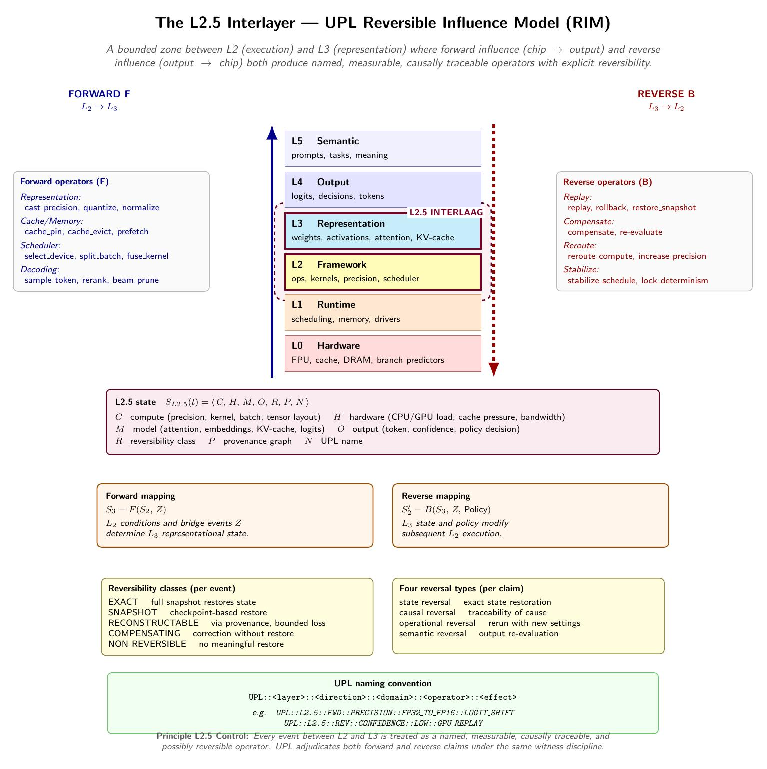
\includegraphics[width=0.98\textwidth]{upl_rim_l2_5_model_v2.pdf}
\caption{The \layer{2}.5 Interlayer --- UPL Reversible Influence
Model (RIM). The bounded zone between \layer{2} (execution) and
\layer{3} (representation) is where forward influence
($\mathrm{chip}\to\mathrm{output}$) and reverse influence
($\mathrm{output}\to\mathrm{chip}$) both produce named, measurable,
causally traceable operators with explicit reversibility. The
L2.5 state $S_{L2.5}(t) = \langle C, H, M, O, R, P, N \rangle$
captures compute, hardware, model, output, reversibility class,
provenance, and UPL name. Forward and reverse mappings share the
same six-witness discipline. Every event between \layer{2} and
\layer{3} is treated as a named, measurable, causally traceable,
and possibly reversible operator (\emph{Principle L2.5\_Control}).}
\label{fig:rim}
\end{figure*}

Figure~\ref{fig:rim} extends the bridge model with explicit
operator structure and bidirectional reversibility. The L2.5
zone is not a new physical layer; it is a bounded reasoning
zone within which forward and reverse claims can be named,
measured, and adjudicated under the same witness discipline.

% ============================================================
\section{Chip-Level Calibrations and Their Propagation}
\label{sec:calibrations}

The bounded-warrant framework is motivated by, but does not
assume, real instances of chip-level conditions affecting model
behaviour. Several configurable \emph{calibrations} are documented
in the literature as inducing observable changes at the model
output. We list them as candidate domains for which the framework
should ultimately be tested.

\paragraph{Mixed-precision arithmetic
(FP32 $\leftrightarrow$ FP16/BF16).}
Mixed-precision training and inference reduce numerical
precision of intermediate values, typically with master-weight
preservation \citep{micikevicius2018}. The chip-level effect is
a change in floating-point rounding behaviour; the L2 effect is
a change in kernel selection; the L3 effect is a perturbation of
activations whose magnitude depends on operator dynamic range.
The witness chain
$\witness{input} \oplus \witness{exec} \oplus \witness{map} \oplus
\witness{contract} \oplus \witness{check} \oplus \witness{ruleout}$
is in principle constructible for any specific input on which the
two precisions diverge in output.

\paragraph{Tensor Float-32 (TF32) on NVIDIA Ampere.}
TF32 \citep{nvidia2020tf32} retains FP32 dynamic range but
truncates the mantissa to 10 bits, accelerating matmul at the
cost of a small precision reduction in the inner-product. TF32 is
enabled by default in PyTorch on Ampere-class hardware unless
explicitly disabled. The configuration --- a single flag in the
runtime --- is a chip-level calibration in the sense developed
here: a property of the execution layer that may or may not be
relevant to a given output boundary.

\paragraph{Deterministic versus non-deterministic kernels.}
Several deep-learning kernels admit multiple implementations that
return numerically distinct outputs on identical inputs due to
non-associativity of floating-point addition under varying
reduction orders \citep{nagarajan2019}. cuDNN, for instance,
exposes a deterministic-mode flag that constrains kernel choice.
The chip-level effect is a change in reduction order; the L3
effect is a perturbation in computed activations; the L4 effect
in rare cases is a flipped classification near decision
boundaries.

\paragraph{Denormal flush-to-zero.}
Many FPUs offer a \emph{flush-to-zero} mode in which subnormal
floating-point values are replaced by zero. The chip-level effect
is a change in rounding behaviour for very small values.
Propagation through \layer{2}--\layer{3} depends on whether
training or inference produces denormals in the relevant operator,
which itself depends on architecture and initialisation.

\paragraph{Memory layout and kernel autotuning.}
Frameworks such as cuDNN run an autotuning phase that selects
kernel implementations based on input shape and device state.
The choice may differ across runs, leading to identical inputs
producing slightly different outputs. The relevant calibration
is at \layer{1}--\layer{2}: the autotuner's selection policy.

\paragraph{Thermal regime and operating temperature.}
A chip's operating temperature $T$ is a continuous calibration
with well-documented influence on lower-layer error rates.
Two physical mechanisms apply. First, Johnson--Nyquist noise gives
a thermal floor on the voltage fluctuation across any resistive
element of resistance $R$ in bandwidth $B$:
\begin{equation}
\langle v_n^2 \rangle \;=\; 4 k_B T R B,
\label{eq:johnson}
\end{equation}
where $k_B$ is the Boltzmann constant. Higher $T$ raises the noise
floor, reducing margin against signal-discrimination errors.
Second, thermally activated failure rates --- charge-leakage,
single-event upsets, and certain refresh-related DRAM errors ---
follow an Arrhenius dependence:
\begin{equation}
\lambda(T) \;=\; \lambda_0 \, \exp\!\left(-\frac{E_a}{k_B T}\right),
\label{eq:arrhenius}
\end{equation}
where $\lambda_0$ is a baseline rate and $E_a$ is the activation
energy of the relevant failure mode. Large-scale field studies of
production DRAM \citep{schroeder2009} confirm that error rates rise
strongly with operating temperature, and architectural studies
have documented disturbance-error mechanisms whose rate depends on
both temperature and access pattern \citep{kim2014}. Within the
present framework, $T$ is a chip-level calibration whose
configuration is partially within operator control (cooling,
workload placement, throttling policy) and partially outside it
(ambient temperature, transient bursts). A layer-effect claim that
implicates a thermal regime would require $\witness{exec}$ to
include a temperature trace and $\witness{ruleout}$ to exclude
attribution to concurrent calibrations.

\medskip

Each calibration above is, in UPL terms, a hypothesis about a
candidate signal. None is here claimed to be a witnessed,
mapped, checked, and ruled-out cause of any specific AI behaviour
under any specific boundary. The contribution of this paper is
the vocabulary in which such claims could be made and adjudicated.
The bounded foundational claim of UPL \citep{hooker2020,
sculley2015} is precisely that: for specific behaviours, under
stated boundaries, with explicit mapping and check, a chip-level
trace \emph{can} be made claim-bearing for an upper-layer output.
The reduction is local, bounded, witnessed.

% ============================================================
\section{Postulates of Reverse Inference and Toy-AI Feedback}
\label{sec:reverse}

The framework presented so far runs in the forward direction:
from a stated chip-level calibration $\witness{exec}$ through the
bridge to an upper-layer output boundary $\witness{check}$.
Two symmetric questions arise. The first concerns
\emph{reverse inference} --- tracing from an observed AI anomaly
back to a candidate chip-level cause. The second concerns
\emph{toy-AI feedback} --- the observation that a small, controlled
AI computation itself produces a measurable signature at the chip
level, which provides an empirical entry point to the framework.

\subsection{Reverse inference}

\begin{quote}\itshape
Given an observed anomaly at the AI output boundary, can the same
witness vocabulary be used in reverse, to identify a candidate
chip-level execution condition that may have produced it?
\end{quote}

We do not assume this is possible in general. We postulate it
as a research direction, subject to the same bounded-warrant
discipline as the forward direction.

\begin{postulate}[Reverse inference]\label{post:reverse}
Let $K^*$ be a claim of the form ``output anomaly $A$ at
\layer{4} was carried by chip-level condition $c \in \mathcal{C}$''
where $\mathcal{C}$ is a finite catalogue of candidate
calibrations. Then under appropriate assumptions $\Gamma$, a
reverse-direction UPL judgment
\[
\Gamma \;\vdash\; K^* \;@\; B \;\Leftarrow\;
\bigl(\witness{anomaly} \oplus \witness{exec}^{*} \oplus \witness{map}^{*} \oplus \witness{contract} \oplus \witness{check}^{*} \oplus \witness{ruleout}^{*}\bigr)
\;:\; \sigma
\]
may be adjudicated with the same status vocabulary
$\Sigma$ as the forward direction, provided:
\begin{itemize}
\item the anomaly is observable at \layer{4} (or higher) and
admits a stated boundary $B$;
\item the candidate catalogue $\mathcal{C}$ is finite, enumerated,
and disjoint;
\item the inverse map $\witness{map}^*$ can be constructed from
\layer{3} representational state back to a specific candidate
$c \in \mathcal{C}$;
\item $\witness{ruleout}^*$ excludes the remaining candidates in
$\mathcal{C} \setminus \{c\}$ under $B$.
\end{itemize}
\end{postulate}

A useful concrete form for $\witness{map}^*$ is Bayesian. If
$\mathcal{C} = \{c_1, \ldots, c_n\}$ with prior $\Pr(c_i)$, the
posterior over candidates given the observed anomaly $A$ is
\begin{equation}
\Pr(c_i \mid A, \Gamma, B)
\;=\;
\frac{\Pr(A \mid c_i, \Gamma, B) \, \Pr(c_i)}
     {\sum_{j=1}^{n} \Pr(A \mid c_j, \Gamma, B) \, \Pr(c_j)}.
\label{eq:bayes}
\end{equation}
A reverse-direction judgment reaches \statuslabel{checked} for
candidate $c_i$ when the posterior concentrates on $c_i$ above a
stated threshold, and when $\witness{ruleout}^*$ supplies witnesses
that the remaining candidates are excluded under $B$. Equation
\eqref{eq:bayes} is not a procedure but a constraint on what
counts as a defensible reverse-inference judgment.

The postulate is consequential. It says the bounded-warrant
framework is in principle bi-directional, even though the
information-theoretic challenges are asymmetric. Forward
inference faces the data-processing inequality
\eqref{eq:dpi}: information may be lost in propagation, so a
strong chip-level signal may not survive to be witnessed at
\layer{4}. Reverse inference faces non-identifiability: many
chip-level events may produce the same observable anomaly, so
$\witness{ruleout}^*$ must work harder.

Reverse inference connects naturally to causal-inference
frameworks \citep{pearl2009} and to the literature on
information-flow tracking in security \citep{kocher2019}.
We do not extend the formal connection in this paper.
We note only that the bounded-warrant vocabulary is symmetric in
form, and asymmetric only in the difficulty of constructing the
required witnesses.

\subsection{Toy-AI feedback as an empirical entry point}
\label{sec:toyai}

Reverse inference (Postulate~\ref{post:reverse}) carries a
constructive obstacle: how is $\witness{map}^*$ to be defined in
practice? The forward direction draws on hardware counters and
framework instrumentation; the reverse direction needs a procedure
that takes an observed output anomaly and produces a posterior
over chip-level candidates. We postulate that the simplest tractable
setting in which this map is constructible is the case of a
deterministic toy AI.

\begin{postulate}[Toy-AI feedback]\label{post:toyai}
Let $\mathcal{M}$ be a deterministic, fully specified
computation --- a \emph{toy AI} --- confined within hardware
boundary $B$. Let $X_3(\mathcal{M}, t)$ denote $\mathcal{M}$'s
\layer{3} representational state at time $t$, and let
$S(\mathcal{M}, t) \in \mathcal{S}$ denote the chip-level
signature produced as a by-product of $\mathcal{M}$'s execution
--- comprising thermal trajectory, instantaneous power draw,
performance-counter readings, cache footprint, and memory-bus
timing. Then under appropriate $\Gamma$ and over a stated horizon,
\begin{equation}
I\bigl(S(\mathcal{M}, t)\,;\, X_3(\mathcal{M}, t) \,\big|\, \Gamma, B\bigr) \;>\; 0.
\label{eq:toyai}
\end{equation}
\end{postulate}

The postulate asserts that the chip-level signature is
non-trivially informative about the toy AI's internal state.
This is not a strong claim --- the right-hand side need not be
large --- but it is sufficient to make reverse inference
non-vacuous in at least one setting. By Fano's inequality
\eqref{eq:fano} applied in the reverse direction, a non-zero
mutual information lower-bounds the achievable adjudication
accuracy from below; conversely, an instrumented toy-AI setting
provides a concrete construction of $\witness{exec}^*$,
$\witness{map}^*$, and ultimately $\witness{ruleout}^*$.

The toy-AI setting is empirically tractable in a way that
production-scale systems are not. The model is small enough to be
fully characterised; the hardware boundary $B$ is small enough to
be instrumented; the computation is deterministic enough that
repeated execution yields a statistical estimate of
$I(S; X_3)$. The framework's reverse-inference postulate is
therefore reduced, in its first instantiation, to a controlled
measurement problem: can a chip-level signature be shown to
carry $\tau$ bits of information about a toy AI's
representational state within stated $B$?

\begin{remark}
Postulate~\ref{post:toyai} does not assume the converse for
production systems. Scaling from toy-AI feedback to bounded
reverse inference on production AI is left open. The postulate
serves as the framework's empirical entry point, not as a
universal claim.
\end{remark}

% ============================================================
\section{Discussion}
\label{sec:discussion}

\paragraph{Scope and first witnessed instance.}
This paper presents the framework within which layer-effect
claims can be made. The next research step described in
earlier drafts --- the construction of a single, fully
witnessed instance of a layer-effect claim across the
\layer{2}--\layer{3} bridge --- has now been executed.

Under a local-machine, single-venv boundary using PyTorch
2.12.0 and a deterministic toy binary linear classifier
($d = 16$), same-precision determinism held in both fp32
and fp16. The cross-precision contrast yielded zero control
flips and one margin flip. Under the declared boundary $B$,
the UPL layer-effect claim
\begin{quote}\itshape\small
``Changing only the execution precision from fp32 to fp16
in the \layer{2} dot-product operation changes the measured
margin representation $z = \mathbf{w}\cdot\mathbf{x} + b$
enough to cross the predefined binary decision boundary for
at least one input in $X_{\mathrm{margin}}$, while
$X_{\mathrm{control}}$ remains invariant''
\end{quote}
was adjudicated with $\sigma = \statuslabel{checked}$. The
full witness chain
$\bigl(\witness{input} \oplus \witness{exec} \oplus
\witness{map} \oplus \witness{contract} \oplus \witness{check}
\oplus \witness{ruleout}\bigr)$
is available in the project repository~\cite{vasen2026demo06}.

This establishes the feasibility of the UPL witness discipline
in a toy precision-contrast setting. It does not establish
broader claims about large language models, production AI
systems, or hardware behaviour generally. The bounding is
intentional and follows directly from the framework's
discipline.

\paragraph{Relation to existing fields.}
UPL is not an AI safety framework. It is not a chip security
framework. It is a provenance vocabulary that may inform both.
AI safety has tools for talking about output behaviour; chip
security has tools for talking about microarchitectural state.
Neither field, at present, has a vocabulary for adjudicating
claims that link the two. This paper proposes one. Whether the
vocabulary is adopted depends on whether the bounded warrants it
demands can in fact be constructed.

\paragraph{What this paper does not claim.}
The framework does not assume that chip-level conditions matter
for AI semantics. It does not assert that any specific calibration
in Section~\ref{sec:calibrations} causes any specific behaviour
under any specific boundary. It does not claim that reverse
inference is achievable in any specific case. It claims only that
a bounded vocabulary exists in which such claims could be stated,
adjudicated, and limited.

\paragraph{Open questions.}
At least four:
\begin{itemize}
\item What measurement instruments can construct $\witness{map}$
across the L2--L3 bridge for current production frameworks?
\item Under what conditions is $\witness{ruleout}$
constructible without exhaustive enumeration of $\mathcal{C}$?
\item How does the framework compose across multiple bridges
(e.g.\ \layer{0}-\layer{2} and \layer{2}-\layer{3} jointly)?
\item Does the reverse-inference postulate
(Postulate~\ref{post:reverse}) admit a constructive proof
under bounded assumptions, or does it require
case-by-case argument?
\end{itemize}

\paragraph{A note on terminology.}
We have deliberately avoided the language of \emph{fault},
\emph{attack}, and \emph{breach} throughout. These terms carry
witness commitments that the present framework does not yet
support. A fault asserts a failure of specification; an attack
asserts intent and control; a breach asserts a witnessed
crossing of a security boundary. The framework presented here
talks instead of \emph{execution conditions}, \emph{candidate
signals}, and \emph{layer-effect claims}. The terminological
restraint is part of the bounded-warrant discipline.

% ============================================================
\section*{Acknowledgements}

This work proceeds in the spirit of small, clean, safe,
understandable infrastructure that has marked Andrew Tanenbaum's
contributions to operating systems pedagogy. Errors and infelicities
remain the author's own.

% ============================================================
\bibliography{references}

\end{document}
